\documentclass[../../main/main.tex]{subfiles}
\graphicspath{{./figures/}}

\dominitoc
\faketableofcontents

\renewcommand{\mtcSfont}{\small\bfseries}
\renewcommand{\mtcSSfont}{\footnotesize}
\mtcsettitle{minitoc}{}
\mtcsetrules{*}{off}

\makeatletter
\renewcommand{\@chapapp}{Induction -- chapitre}
\makeatother

% \toggletrue{student}
% \toggletrue{corrige}
% \renewcommand{\mycol}{black}
% \renewcommand{\mycol}{gray}

\hfuzz=5.003pt

\begin{document}
\setcounter{chapter}{2}

\settype{book}
\settype{prof}
\settype{stud}

\chapter{Lois de l'induction et induction de \textsc{Neumann}}
\label{ch:loisinduc}
% \epigraph{\openquote\textit{%
% 		Sire, je n'avais pas besoin de cette hypothèse.
% 	}%
% 	\closequote}{Pierre-Simon \textsc{Laplace} à \textsc{Napoléon}, \textit{circa} 1800}

\vspace*{\fill}

\begin{tcn}(appl)<ctc>"somm"'t'{Sommaire}
	\let\item\olditem
	\vspace{-15pt}
	\minitoc
	\vspace{-25pt}
\end{tcn}

\begin{tcn}[sidebyside, fontupper=\small, fontlower=\small](appl)<ctb>"how"'t'{Capacités exigibles}
	\begin{itemize}[label=\rcheck]
		\item Évaluer le flux d'un champ magnétique uniforme à travers une surface
		      s'appuyant sur un contour fermé orienté plan.

		\item Utiliser la loi de \textsc{Lenz} pour prédire ou interpréter les
		      phénomènes physiques observés.

		\item Utiliser la loi de \textsc{Faraday} en précisant les conventions
		      d'algébrisation

		\item Différencier le flux propre des flux extérieurs. Utiliser la loi de
		      modération de \textsc{Lenz}.

		\item Évaluer et citer l'ordre de grandeur de l'inductance propre d'une
		      bobine de grande longueur.
	\end{itemize}
	\tcblower
	\begin{itemize}[label=\rcheck]
		\item Réaliser un bilan de puissance et d'énergie dans un système siège d'un
		      phénomène d'auto-induction en s'appuyant sur un schéma électrique
		      équivalent.

		\item Déterminer l'inductance mutuelle entre deux bobines de même axe de
		      grande longueur en «~influence totale~»

		\item Citer des applications dans le domaine de l'industrie ou de la vie
		      courante.

		\item Établir le système d'équations en régime sinusoïdal forcé en
		      s'appuyant sur des schémas électriques équivalents.

		\item Réaliser un bilan de puissance et d'énergie.
	\end{itemize}
\end{tcn}

% \vspace{-15pt}

\vspace*{\fill}

\newpage

\vspace*{\fill}
% {%
% \begin{boxes}
\begin{tcn}[sidebyside, fontupper=\small, fontlower=\small](appl)<ctb>"chek"'t'{L'essentiel}
	% \begin{tcn}(defi)<ctc>'t'{Définitions}
	% 	\tcblistof[\paragraph*]{defi}{\hspace*{4.8pt}}
	% \end{tcn}
	% \begin{tcn}(rapp)<ctc>'t'{Rappels}
	% 	\tcblistof[\paragraph*]{rapp}{\hspace*{4.8pt}}
	% \end{tcn}
	\begin{tcn}(prop)<ctc>'t'{Propriétés}
		\tcblistof[\paragraph*]{prop}{\hspace*{4.8pt}}
		\tcblistof[\paragraph*]{loi}{\hspace*{4.8pt}}
		% \tcblistof[\paragraph*]{theo}{\hspace*{4.8pt}}
	\end{tcn}
	% \begin{tcn}(coro)<ctc>'t'{Corollaires}
	%   \tcblistof[\paragraph*]{coro}{\hspace*{4.8pt}}
	% \end{tcn}
	\begin{tcn}(demo)<ctc>'t'{Démonstrations}
		\tcblistof[\paragraph*]{demo}{\hspace*{4.8pt}}
		\tcblistof[\paragraph*]{prev}{\hspace*{4.8pt}}
	\end{tcn}
	% \begin{tcn}(inte)<ctc>'t'{Interprétations}
	% 	\tcblistof[\paragraph*]{inte}{\hspace*{4.8pt}}
	% \end{tcn}
	\begin{tcn}(impl)<ctc>'t'{Implications}
		\tcblistof[\paragraph*]{impl}{\hspace*{4.8pt}}
	\end{tcn}
	% \begin{tcn}(tool)<ctc>'t'{Outils}
	% 	\tcblistof[\paragraph*]{tool}{\hspace*{4.8pt}}
	% \end{tcn}
	% \begin{tcn}(nota)<ctc>'t'{Notations}
	%   \tcblistof[\paragraph*]{nota}{\hspace*{4.8pt}}
	% \end{tcn}
	% \begin{tcn}(appl)<ctc>'t'{Applications}
	% 	\tcblistof[\paragraph*]{appl}{\hspace*{4.8pt}}
	% \end{tcn}
	% \begin{tcn}(rema)<ctc>'t'{Remarques}
	%   \tcblistof[\paragraph*]{rema}{\hspace*{4.8pt}}
	% \end{tcn}
	\begin{tcn}(exem)<ctc>'t'{Exemples}
		\tcblistof[\paragraph*]{exem}{\hspace*{4.8pt}}
	\end{tcn}
	% \begin{tcn}*(ror)<ctc>"hart"'t'{Points importants}
	%   \tcblistof[\paragraph*]{ror}{\hspace*{4.8pt}}
	% \end{tcn}
	% \begin{tcn}(impo)<ctc>'t'{Erreurs communes}
	%   \tcblistof[\paragraph*]{impo}{\hspace*{4.8pt}}
	% \end{tcn}
	\tcblower
	% \begin{tcn}(defi)<ctc>'t'{Définitions}
	%   \tcblistof[\paragraph*]{defi}{\hspace*{4.8pt}}
	% \end{tcn}
	% \begin{tcn}(rapp)<ctc>'t'{Rappels}
	%   \tcblistof[\paragraph*]{rapp}{\hspace*{4.8pt}}
	% \end{tcn}
	% \begin{tcn}(prop)<ctc>'t'{Propriétés}
	%   \tcblistof[\paragraph*]{prop}{\hspace*{4.8pt}}
	%   \tcblistof[\paragraph*]{loi}{\hspace*{4.8pt}}
	%   \tcblistof[\paragraph*]{theo}{\hspace*{4.8pt}}
	% \end{tcn}
	% \begin{tcn}(coro)<ctc>'t'{Corollaires}
	%   \tcblistof[\paragraph*]{coro}{\hspace*{4.8pt}}
	% \end{tcn}
	% \begin{tcn}(demo)<ctc>'t'{Démonstrations}
	% 	\tcblistof[\paragraph*]{demo}{\hspace*{4.8pt}}
	% 	\tcblistof[\paragraph*]{prev}{\hspace*{4.8pt}}
	% \end{tcn}
	% \begin{tcn}(inte)<ctc>'t'{Interprétations}
	% 	\tcblistof[\paragraph*]{inte}{\hspace*{4.8pt}}
	% \end{tcn}
	% \begin{tcn}(impl)<ctc>'t'{Implications}
	% 	\tcblistof[\paragraph*]{impl}{\hspace*{4.8pt}}
	% \end{tcn}
	% \begin{tcn}(tool)<ctc>'t'{Outils}
	%   \tcblistof[\paragraph*]{tool}{\hspace*{4.8pt}}
	% \end{tcn}
	% \begin{tcn}(nota)<ctc>'t'{Notations}
	%   \tcblistof[\paragraph*]{nota}{\hspace*{4.8pt}}
	% \end{tcn}
	% \begin{tcn}(odgr)<ctc>'t'{Ordres de grandeur}
	% 	\tcblistof[\paragraph*]{odgr}{\hspace*{4.8pt}}
	% \end{tcn}
	\begin{tcn}(appl)<ctc>'t'{Applications}
		\tcblistof[\paragraph*]{appl}{\hspace*{4.8pt}}
	\end{tcn}
	% \begin{tcn}(rema)<ctc>'t'{Remarques}
	%   \tcblistof[\paragraph*]{rema}{\hspace*{4.8pt}}
	% \end{tcn}
	% \begin{tcn}(exem)<ctc>'t'{Exemples}
	% 	\tcblistof[\paragraph*]{exem}{\hspace*{4.8pt}}
	% \end{tcn}
	\begin{tcn}*(ror)<ctc>"hart"'t'{Points importants}
		\tcblistof[\paragraph*]{ror}{\hspace*{4.8pt}}
	\end{tcn}
	\begin{tcn}(impo)<ctc>'t'{Erreurs communes}
		\tcblistof[\paragraph*]{impo}{\hspace*{4.8pt}}
	\end{tcn}
\end{tcn}
% \end{boxes}
% }%

\vspace*{\fill}
\newpage

% Dans les chapitres précédents, nous avons vu que le passage d'un courant
% électrique dans un circuit entraînait la création d'un champ magnétique. Ici
% nous étudions la situation opposée~: un champ magnétique peut entraîner la
% création d'un courant électrique.

\section{Le phénomène d'induction}
\label{sec:phinduc}
\subsection{Observations expérimentales}
\label{ssec:inducobsexp}

Soit un solénoïde (bobine longue) non alimenté, relié à un ampèremètre mesurant
le courant qui le traverse. On étudie sa réaction à un champ magnétique dans
deux situations\footnote{Voir l'animation~:
	\url{https://phet.colorado.edu/sims/html/faradays-law/latest/faradays-law_fr.html}}~:

\begin{tcb}(expe)<lftt>{Bobine dans des champs magnétiques}
	\tcbsubtitle{\fatbox{\textbf{Champ magnétique constant}}}
	\begin{isd}
		\begin{center}
			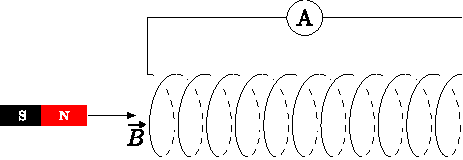
\includegraphics[width=\linewidth]{inducexp1}
			\label{fig:inducexp1}
		\end{center}
		\tcblower
		Les lignes de champ d'un aimant vont de sont Nord vers son Sud. Un champ
		magnétique règne donc dans le solénoïde. On n'observe cependant aucun courant
		dans le solénoïde.
	\end{isd}
	\tcblower
	\tcbsubtitle{\fatbox{\textbf{Champ magnétique variable}}}
	\begin{isd}
		\begin{center}
			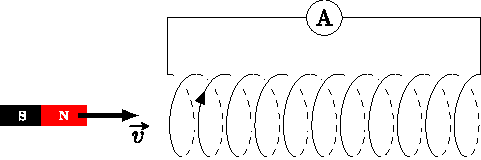
\includegraphics[width=\linewidth]{inducexp2}
			\label{fig:inducexp2}
		\end{center}
		\tcblower
		On déplace l'aimant à proximité de la bobine. On constate qu'\textbf{un
			courant apparaît} dans la bobine, malgré l'absence de générateur.
	\end{isd}
\end{tcb}

% \paragraph*{Bobine dans un champ magnétique constant}~
% \smallbreak
%
% \noindent
% \begin{minipage}[t]{.4\linewidth}
% 	~
% 	\vspace*{-25pt}
% 	\begin{center}
% 		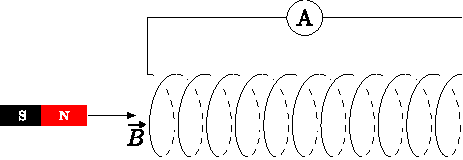
\includegraphics[width=\linewidth]{inducexp1}
% 		\label{fig:inducexp1}
% 	\end{center}
% \end{minipage}
% \hfill
% \begin{minipage}[t]{.55\linewidth}
% 	Les lignes de champ d'un aimant vont de sont Nord vers son Sud. Un champ
% 	magnétique règne donc dans le solénoïde. On n'observe cependant aucun courant
% 	dans le solénoïde.
% \end{minipage}
%
% \paragraph*{Bobine dans un champ magnétique variable}~
% \smallbreak
%
% \noindent
% \begin{minipage}[t]{.4\linewidth}
% 	~
% 	\vspace*{-25pt}
% 	\begin{center}
% 		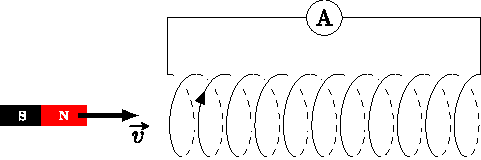
\includegraphics[width=\linewidth]{inducexp2}
% 		\label{fig:inducexp2}
% 	\end{center}
% \end{minipage}
% \hfill
% \begin{minipage}[t]{.55\linewidth}
% 	On déplace l'aimant à proximité de la bobine. On constate qu'\textbf{un
% 		courant apparaît} dans la bobine, malgré l'absence de générateur.
% \end{minipage}

\begin{tcb}(obsv)<lftt>{Bobine et champs magnétiques}
	En étudiant le sens du courant induit, on observe que le sens de déplacement de
	l'aimant et du courant sont liés~:
	\smallbreak
	\begin{isd}
		\begin{itemize}
			\item \psw{%
				      Sans mouvement relatif, pas de courant
			      }%
			\item \psw{%
				      Si on approche l'aimant ou le circuit, $i > 0$
			      }%
			\item \psw{%
				      Si on éloigne l'aimant ou le circuit, $i < 0$
			      }%
		\end{itemize}
		\tcblower
		\begin{itemize}
			\item \psw{%
				      Si on retourne l'aimant, le courant est opposé
			      }%
			\item \psw{%
				      Plus le mouvement est rapide, plus le courant généré est grand
			      }%
		\end{itemize}
	\end{isd}
\end{tcb}

% \subsection{Bilan}
% \label{ssec:inducexpbilan}

\begin{tcb*}(defi){Induction électromagnétique}
	Le phénomène d'induction électromagnétique est l'apparition d'une
	\textbf{tension} électrique (et donc à un \textbf{courant} si le circuit est
	fermé) dans un circuit soumis à un champ magnétique dans deux cas de figure~:
	\begin{enumerate}
		\item \psw{%
			      Lorsque le circuit est plongé dans un champ magnétique
			      \textbf{variable}~: induction de \textsc{Neumann}~;
		      }%
		\item \psw{%
			      Lorsque le circuit est \textbf{déformé} dans un champ magnétique
			      constant~: induction de \textsc{Lorentz} (voir chapitre suivant).
		      }%
	\end{enumerate}
\end{tcb*}

% \begin{tcb*}(exem)<lft>'l'{Application}
% 	Dans chacun des circuits ci-dessous, la spire circulaire et/ou l'aimant droit
% 	sont déplacés dans le sens indiqué par la double flèche. Indiquer le signe du
% 	courant $i$ apparaissant dans la spire pendant le déplacement.
% 	\begin{center}
% 		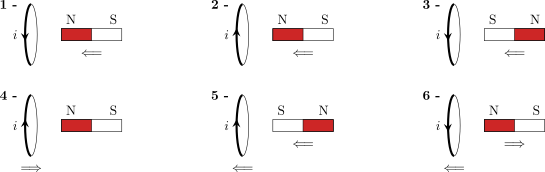
\includegraphics[scale=1]{inducsigne}
% 		\label{fig:inducsigne}
% 	\end{center}
% 	\tcblower
% 	\psw{%
% 		Les lignes de champ vont du Nord vers le Sud. On doit déterminer le sens de
% 		variation du champ vu par la spire~: le champ induit atténue cette variation.
% 		On en déduit le signe réel de $i$ par la règle de la main droite.
% 		\smallbreak
% 	}%
% 	\begin{isd}
% 		\psw{%
% 			\begin{enumerate}
% 				\item
% 				      $\vv{B}_{\rm aimant}$ augmente vers la gauche~: $\vv{B}_{\rm
% 						      induit}$ est vers la droite, donc issu de $i\ind{ind} > 0$.
% 				      \begin{center}
% 					      \sswitch{%
% 						      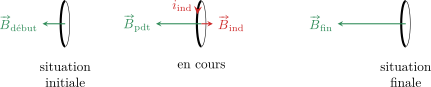
\includegraphics[width=\linewidth, draft=true]{inducsigne_a}
% 						      \label{fig:indsa}
% 					      }{%
% 						      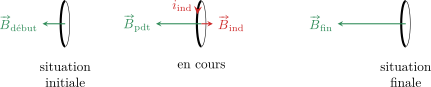
\includegraphics[width=\linewidth]{inducsigne_a}
% 						      \label{fig:indsa}
% 					      }%
% 				      \end{center}
% 				\item
% 				      Même situation physique, convention opposée~: $i\ind{ind} < 0$.
% 				\item
% 				      Cette fois $\vv{B}_{\rm aimant}$ augmente vers la droite~:
% 				      $\vv{B}\ind{ind}$ est vers la gauche. Sens réel du courant opposé~:
% 				      $i\ind{ind} < 0$.
% 				      \begin{center}
% 					      \sswitch{%
% 						      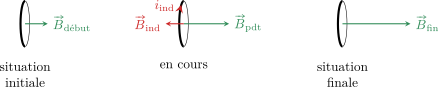
\includegraphics[width=\linewidth, draft=true]{inducsigne_b}
% 						      \label{fig:indsb}
% 					      }{%
% 						      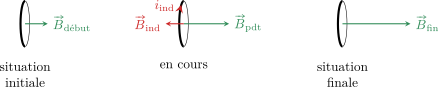
\includegraphics[width=\linewidth]{inducsigne_b}
% 						      \label{fig:indsb}
% 					      }%
% 				      \end{center}
% 			\end{enumerate}
% 		}%
% 		\tcblower
% 		\psw{%
% 			\begin{enumerate}[start=4]
% 				\item \psw{%
% 					      Pareil qu'à la question 2~: $i\ind{ind} < 0$.
% 				      }%
% 				\item \psw{%
% 					      Pas de mouvement relatif donc pas de variation de champ donc pas
% 					      d'induction~: $i\ind{ind} = 0$.
% 				      }%
% 				\item \psw{%
% 					      Mouvement relatif amplifié. Ici, le champ \textbf{diminue} vers la
% 					      gauche, donc le champ induit le \textbf{renforce}~; ainsi $i\ind{ind} <
% 						      0$.
% 				      }%
% 				      \begin{center}
% 					      \sswitch{%
% 						      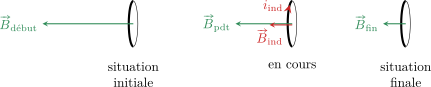
\includegraphics[width=\linewidth, draft=true]{inducsigne_c}
% 						      \label{fig:indsc}
% 					      }{%
% 						      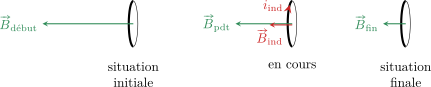
\includegraphics[width=\linewidth]{inducsigne_c}
% 						      \label{fig:indsc}
% 					      }%
% 				      \end{center}
% 			\end{enumerate}
% 		}%
% 	\end{isd}
% \end{tcb*}

\subsection{Flux magnétique}
\label{ssec:flux}
\begin{tcb*}[sidebyside, righthand ratio=.4](defi){Flux magnétique}
	On définit le \textbf{flux du champ magnétique $\Bf$ à travers un circuit}
	comme l'intégrale de $\Bf$ sur la surface \textbf{orientée} entourée par le
	circuit~:
	% Soit $S$ une surface \textbf{plane}, délimitée par un contour
	% \textbf{orienté} par le sens réel du courant, telle que $\vv{S} = S\,\vv{n}$
	% avec $\vv{n}$ unitaire normal au plan de sens lié au courant par la main
	% droite. Soit $\vv{B}(t)$ le champ magnétique \textbf{uniforme} qui la
	% traverse.
	\psw{%
		\[
			\F_S(\vv{B}) = \iint _{\Mr \in S}^{} \dd{\F(\Mr)} = \iint _{\Mr \in S}^{}
			\vv{B}(\Mr)\cdot \dd{\vv{S}(\Mr)}
		\]
	}%
	et si le champ $\Bf$ est \textbf{uniforme} et que le circuit est
	\textbf{une spire}, alors on a
	\psw{%
		\[
			\F_S(\Bf) = \Bf \cdot \vv{S}
			\quad \Ra \quad
			\F_{N~\text{spires}}(\Bf) = N\F_S(\Bf) = N \Bf \cdot \vv{S}
		\]
	}%
	\tcblower
	\begin{center}
		\sswitch{
			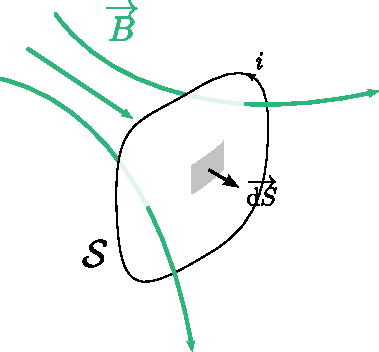
\includegraphics[width=\linewidth, draft=true]{fluxdef_var}
		}{
			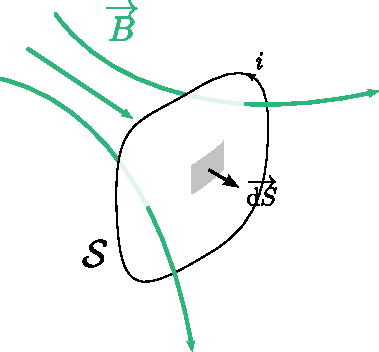
\includegraphics[width=\linewidth]{fluxdef_var}
		}
	\end{center}
	% \smallbreak
	% \noindent
	% \hfill
	% \begin{minipage}[t]{.2\linewidth}
	% 	\begin{center}
	% 		\sswitch{%
	% 			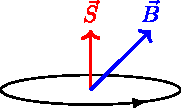
\includegraphics[scale=1, draft=true]{fluxdef}
	% 			\label{fig:fluxdef}
	% 		}{%
	% 			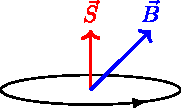
\includegraphics[scale=1]{fluxdef}
	% 			\label{fig:fluxdef}
	% 		}%
	% 	\end{center}
	% 	\hfill
	% \end{minipage}
	% \noindent
	% \begin{minipage}[t]{.2\linewidth}
	% 	\begin{center}
	% 		\sswitch{%
	% 			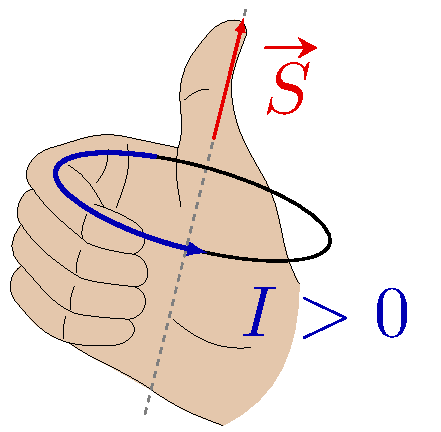
\includegraphics[height=2cm, draft=true]{ra_surface}
	% 			\label{fig:rasurf}
	% 		}{%
	% 			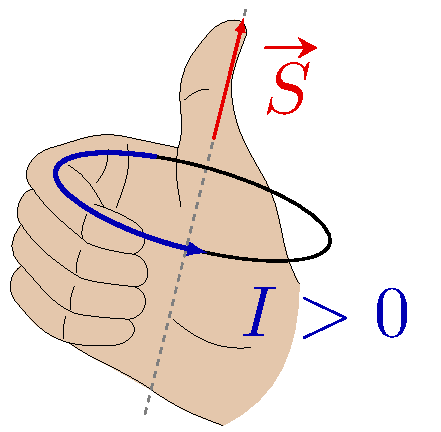
\includegraphics[height=2cm]{ra_surface}
	% 			\label{fig:rasurf}
	% 		}%
	% 	\end{center}
	% \end{minipage}
	% \hfill~
	% \smallbreak
	% \psw{%
	% 	On appelle \textbf{flux} de $\vv{B}$ à travers $S$ la grandeur
	% 	\textbf{scalaire} $\F_S(\vv{B})$ telle que
	% 	\[
	% 		\boxed{\F_S(\vv{B}) = \vv{B}\cdot \vv{S}}
	% 	\]
	% 	\vspace*{-10pt}
	% }%
\end{tcb*}

% \begin{tcb*}(rema)<lft>'l'{}
% 	Au travers de $N$ spires parcourues par le même champ $\vv{B}$, on a
% 	\psw{%
% 		\[
% 			\F(t) = N\times \vv{B}\cdot \vv{S}
% 		\]
% 		\vspace*{-20pt}
% 	}%
% \end{tcb*}

% On se limite à la description des cas où le champ magnétique est
% \textbf{uniforme} à l'échelle de de la situation pour une surface
% \textbf{plane}. Dans un cas plus général, il faudrait effectuer une double
% intégration sur la surface, en la découpant en éléments infinitésimaux
% $\dd{S}(\Mr)$ avec $\Mr \in S$~:
% \[
% 	\F_S(\vv{B}) = \iint _{\Mr \in S}^{} \dd{\F(\Mr)} = \iint _{\Mr \in S}^{}
% 	\vv{B}(\Mr)\cdot \dd{\vv{S}(\Mr)}
% \]

\begin{tcb*}(appl)<lftt>'l'{Calculs simples de flux}
	Déterminer le flux au travers de la spire circulaire de rayon $R$ plongée dans
	$\vv{B}$ uniforme dans les 4 situations suivantes~:
	\begin{center}
		\begin{tabularx}{\linewidth}{Y|Y|Y|Y}
			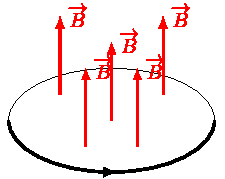
\includegraphics[width=\linewidth]{fluxexo_a} &
			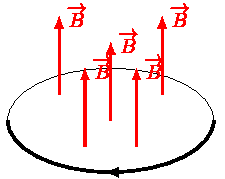
\includegraphics[width=\linewidth]{fluxexo_b} &
			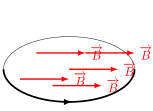
\includegraphics[width=\linewidth]{fluxexo_c} &
			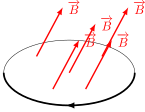
\includegraphics[width=\linewidth]{fluxexo_d}          \\
			\psw{%
				$\vv{S}\cdot \vv{B} > 0 \Ra \F_S(\vv{B}) = BS$
			}%
			                                              &
			\psw{%
				$\vv{S}\cdot \vv{B} < 0 \Ra \F_S(\vv{B}) = -BS$
			}%
			                                              &
			\psw{%
				$\vv{S}\cdot \vv{B} = 0 \Ra \F_S(\vv{B}) = 0$
			}%
			                                              &
			\psw{%
				$\vv{S}\cdot \vv{B} = -BS\cos{\theta} = \F_S(\vv{B})$
			}%
			\\
			                                              &   &  & \\
		\end{tabularx}
	\end{center}
\end{tcb*}

\begin{tcb*}(defi){Flux propre et flux extérieur}
	Puisqu'un circuit électrique est capable de créer un champ \textbf{propre}
	$\Bf_p$ mais peut également être plongé dans un champ \textbf{extérieur}
	$\Bf\ind{ext}$, on distingue les deux flux~:
	\smallbreak
	\begin{isd}
		\tcbsubtitle{\fatbox{Flux propre}}
		\psw{%
			\[
				\F_p = \iint_{S} \Bf_p \cdot \vv{S}
			\]
		}%
		\vspace{-15pt}
		\tcblower
		\tcbsubtitle{\fatbox{Flux extérieur}}
		\psw{%
			\[
				\F\ind{ext} = \iint_{S} \Bf\ind{ext} \cdot \vv{S}
			\]
		}%
		\vspace{-15pt}
	\end{isd}
\end{tcb*}

\subsection{Loi de \textsc{Faraday}}
\label{ssec:fara}
\begin{tcb*}[breakable](prop){Loi de \textsc{Faraday}}
	Soit un circuit électrique \textbf{fermé} et \textbf{orienté par une
		intensité} soumis à l'action d'un champ magnétique $\vv{B}$. Toute
	\textbf{variation du flux} $\F_S(\vv{B})$ dans ce circuit y fait apparaître
	une \textbf{force électromotrice} (tension à vide) induite $e$,
	\textbf{orientée dans le même sens que $i$}, telle que
	\psw{%
		\[
			\boxed{e\ind{ind}(t) =
				-\dv{\F}{t}} = -\dv{t} \iint_{S} \Bf \cdot \dd{S}
		\]
	}%
	Le système se comporte comme si on y avait mis un
	\textbf{générateur électrique} idéal de f.é.m.\ $e$.
	\smallbreak
	% \vspace*{-0pt}
	\hfill
	\noindent
	\begin{minipage}[c]{.4\linewidth}
		~
		\begin{center}
			\sswitch{%
				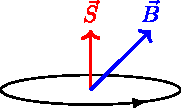
\includegraphics[scale=1, draft=true]{fluxdef}
			}{%
				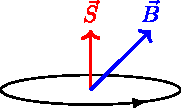
\includegraphics[scale=1]{fluxdef}
			}%
			\label{fig:fluxdef2}
			\smallbreak
			Circuit physique.
			\smallbreak
			$\vv{S}$ \textbf{orientée avec $i$}.
		\end{center}
	\end{minipage}
	\hfill
	\begin{minipage}[c]{.4\linewidth}
		~
		\begin{center}
			\sswitch{%
				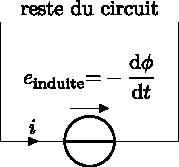
\includegraphics[scale=1, draft=true]{faraelec}
			}{%
				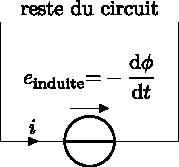
\includegraphics[scale=1]{faraelec}
			}%
			\label{fig:faraelec}
			\smallbreak
			Modèle électrique.
			\smallbreak
			$i\ind{ind}$ et $e\ind{ind}$ \textbf{dans le même sens}.
		\end{center}
	\end{minipage}
	\hfill~
	%
\end{tcb*}

\begin{tcb}(rema)<lftt>'l'{Loi de \textsc{Faraday}}
	\begin{enumerate}
		\item Il y a deux manières de faire varier le flux $\F$~:
		      \begin{itemize}
			      \item[b]{\textsc{Neumann}}: \psw{on fait varier le champ $\Bf$}
			      \item[b]{\textsc{Lorentz}}: \psw{on déforme le circuit}
		      \end{itemize}
		\item \psw{%
			      La f.é.m. $e$ est orientée dans le même sens que le courant $i$, donc
			      en convention \textbf{générateur}~;
		      }%
		\item \psw{%
			      Le signe «~$-$~» donne la loi de \textsc{Lenz}, et découle en fait
			      de la conservation de l'énergie.
		      }%
	\end{enumerate}
\end{tcb}
\vspace{-15pt}

\subsection{Loi de modération de \textsc{Lenz}}

Le sens du courant obtenu est donné par la \textbf{loi de \textsc{Lenz}}~:
\begin{tcb*}[sidebyside, righthand ratio=.25](ror){Loi de modération de \textsc{Lenz}}
	Lorsque le flux extérieur $\F\ind{ext}$ à travers un circuit \textbf{fermé}
	varie, ceci a pour conséquence de faire apparaître une \textbf{intensité dans
		le circuit}, qui a son tour est à l'origine d'un \textbf{champ magnétique
		propre}, dont le flux $\F_p$ \textbf{s'oppose à la variation introduite}. On
	dit souvent~:
	\begin{center}
		\psw{%
			L'induction modère, par ses conséquences, les causes qui lui ont donné
			naissance.
		}%
	\end{center}
	\tcblower
	\begin{center}
		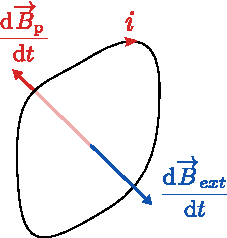
\includegraphics[width=\linewidth]{lenz_prop}
	\end{center}
\end{tcb*}

\begin{tcb*}(exem)<lftt>{Loi de modération de \textsc{Lenz}}
	Prenons un exemple très simple d'une spire plongée initialement sans courant
	dans un champ magnétique $B\ind{ext}$. Supposons que ce champ augmente en
	intensité~:
	\begin{center}
		\sswitch{
			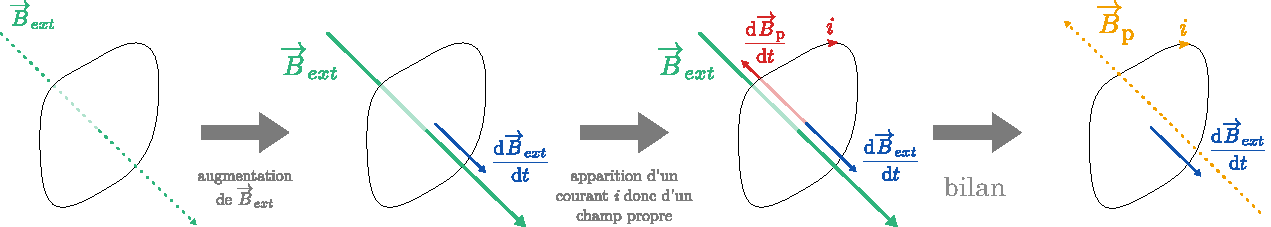
\includegraphics[width=\linewidth, draft=true]{lenz_exem}
		}{
			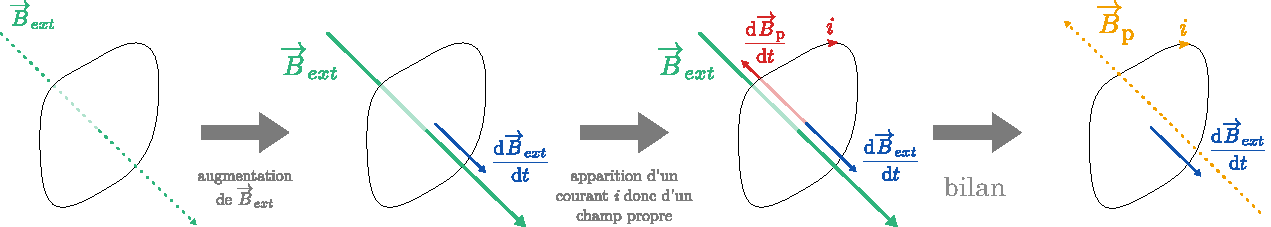
\includegraphics[width=\linewidth]{lenz_exem}
		}
	\end{center}
	Dès que $\Bf\ind{ext}$ arrête d'augmenter, le champ propre précédemment créé
	disparaît.
\end{tcb*}

\begin{itemize}
	\item[b]{\textsc{Neumann}}: courant induit créé un nouveau champ $\vv{B_0}$
	qui contrecarre les \textbf{variations} de $\vv{B\ind{ext}}$ initial~;
	\item[b]{\textsc{Lorentz}}: courant induit créé un nouveau champ $\vv{B_0}$
	qui impose une force s'opposant à la \textbf{déformation}.
\end{itemize}

\begin{tcb*}(appl)<lftt>'l'{\textsc{Lenz} et \textsc{Faraday} circuit carré}
	\noindent
	\begin{minipage}[c]{.75\linewidth}
		On considère un circuit carré de côté $a$ et de résistance totale $R$, situé
		dans un plan orthogonal à un champ magnétique uniforme mais \textbf{variable}
		$\vv{B}(t) = B_0\exr^{-t/\tau}\uz$ avec $B_0$ et $\tau$ strictement positifs.
		Un phénomène d'induction se produit-il dans le circuit~? Si oui, exprimer
		l'intensité $i$ du courant induit représenté sur le schéma, et vérifier que
		son signe soit en accord avec la loi de \textsc{Lenz}.
	\end{minipage}
	\hfill
	\begin{minipage}[c]{.24\linewidth}
		\begin{center}
			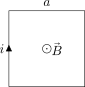
\includegraphics[scale=1]{faraexo}
			\label{fig:faraexo}
		\end{center}
	\end{minipage}
	\tcblower
	\psw{%
		Le flux à travers le circuit de surface $S = a^2$ est variable puisque le
		champ magnétique l'est. Il y a donc un phénomène d'induction. On a alors~:
		\begin{gather*}
			\begin{aligned}{}
				\F_S(\vv{B}) & = -Ba^2
				\\
				             & = -B_0a^2\exr^{-t/\tau}
			\end{aligned}
			\qqso
			\begin{aligned}{}
				e\ind{ind}         & = -\dv{\F}{t}
				\\\Lra
				\Aboxed{e\ind{ind} & = -\frac{B_0a^2}{\tau}\exr^{-t/\tau} < 0}
			\end{aligned}
		\end{gather*}
		Or, comme le circuit est fermé,
		\begin{align*}
			e\ind{ind}         & = Ri\ind{ind}
			\\\Lra
			\Aboxed{i\ind{ind} & = -\frac{B_0a^2}{R\tau}\exr^{-t/\tau} < 0}
		\end{align*}
		donc l'intensité est \textbf{négative}. En effet, le champ magnétique induit
		réel doit s'opposer à la diminution du champ extérieur $\vv{B}$, en créant un
		champ magnétique positif selon $\uz$~: le sens réel du courant donné par la
		main droite est l'opposé de celui représenté.
		\vspace*{-10pt}
	}%
\end{tcb*}

\section{Phénomène d'autoinduction}
\label{sec:autoind}

\subsection{Champs propre et extérieur}
\label{ssec:fpropre}
Lorsqu'un courant circule dans une bobine, il créé un champ magnétique. Or, ce
champ créé contribue au flux magnétique total à travers le circuit, et génère
une force électromotrice d'induction~:
\begin{tcb}(defi){Champ magnétique total}
	Lors de l'étude de l'induction dans un circuit, on différencie le champ créé
	par le circuit, dit \textbf{champ propre}, des autres champs issus d'autres
	sources~:
	\psw{%
		\[
			\boxed{\vv{B\ind{tot}} = \vv{B\ind{propre}} + \vv{B\ind{ext}}}
		\]
	}%
	\vspace*{-10pt}
\end{tcb}
\begin{tcb}(rapp){Champ d'une bobine}
	Pour une bobine, le champ magnétique propre est celui créé par le courant que
	nous avons déjà vu~:
	\psw{%
		\[
			\vv{B\ind{p}}(t) = \mu_0 \frac{N}{\ell }i(t)\,\uz
		\]
	}%
\end{tcb}

Le champ magnétique extérieur est lié à la présence d'autres sources au
voisinage (champs de fils électriques par exemple.)

% \begin{tcb*}(defi){Flux propre}
% 	\noindent
% 	\begin{minipage}[t]{.7\linewidth}
% 		\begin{center}
% 			\psw{%
% 				On appelle \textbf{flux propre} noté $\F_p$ d'un circuit le flux de son
% 				champ magnétique propre $\vv{B_p}$ à travers lui-même.
% 				% \bigbreak
% 				% \begin{tcn}[width=.8\linewidth](impo){Attention}
% 				% 	$\F_p \neq \vv{B_p}\cdot \vv{S}$ car \textbf{le champ propre
% 				% 		n'est pas uniforme}
% 				% \end{tcn}
% 			}%
% 		\end{center}
% 	\end{minipage}
% 	\hfill
% 	\begin{minipage}[t]{.29\linewidth}
% 		~
% 		\vspace*{-20pt}
% 		\begin{center}
% 			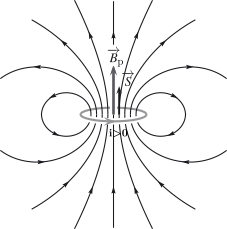
\includegraphics[height=2cm]{fpropre}
% 			\label{fig:fpropre}
% 		\end{center}
% 	\end{minipage}
% \end{tcb*}

\subsection{Auto-inductance}
\label{ssec:autoind}
\begin{tcb*}[sidebyside, righthand ratio=.35](prop){Auto-inductance d'un circuit}
	On admet que le flux propre dans un circuit est \textbf{proportionnel à
		l'intensité} du courant dans le circuit, tel que
	\psw{%
		\[
			\boxed{\F_p(t) = Li(t)}
		\]
	}%
	avec $L$ l'\textbf{inductance propre} (ou auto-inductance) du circuit.
	\begin{itemize}
		\item \psw{%
			      $L > 0$ car $i$ et $\vv{B_p}$ sont orientés par la main droite.
		      }%
		\item \psw{%
			      $L$ ne dépend que de la \textbf{taille} et \textbf{forme} du circuit.
		      }%
		\item \psw{%
			      $L$ s'exprime en henry (\si{H}).
		      }%
	\end{itemize}
	\tcblower
	\begin{center}
		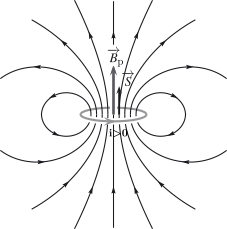
\includegraphics[width=\linewidth]{fpropre}
		\label{fig:fpropre}
	\end{center}
\end{tcb*}

\begin{tcb*}[breakable](appl)<lftt>'l'{Inductance propre d'une bobine}
	Calcul de l'inductance propre d'une bobine. On donne le champ propre
	$\vv{B_p}$ créé dans un solénoïde~:
	\[
		\vv{B_p}(t) = \mu_0 \frac{N}{\ell }i(t)\,\uz
	\]
	\begin{enumerate}
		\item Le sens du courant étant donné, indiquer le sens du champ magnétique.
		      \smallbreak
		      \noindent
		      \begin{minipage}[c]{.4\linewidth}
			      \begin{center}
				      \sswitch{%
					      
\includegraphics[scale=1]{bobi}
					      \label{fig:bobib}
				      }{%
					      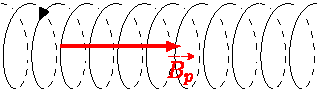
\includegraphics[scale=1]{bobib}
					      \label{fig:bobi}
				      }%
			      \end{center}
		      \end{minipage}
		      \hfill
		      \begin{minipage}[c]{.69\linewidth}
			      \psw{%
				      $i$ et $\vv{B_p}$ respectent la règle de la main droite.
			      }%
		      \end{minipage}
		\item Exprimer le flux du champ magnétique.
		      \smallbreak
		      \psw{%
			      Pour $N$ spires~:
			      \[
				      \F_p = N\times \vv{B_p}\cdot \vv{S}
			      \]
			      Or, $\vv{B_p}$ et $\vv{S}$ sont tous deux orientés à partir de $i$
			      selon la règle de la main droite, donc
			      \begin{gather*}
				      \vv{S} = S\uz
				      \qqet
				      \vv{B_p} = \mu_0 \frac{N}{\ell }i(t)\,\uz
				      \\\Lra
				      \boxed{\F_p = \mu_0 \frac{N^2}{\ell }Si(t)}
			      \end{gather*}
		      }%
		\item En déduire l'expression de l'inductance propre.
		      \psw{%
			      On a démontré que le flux magnétique propre et l'intensité étaient
			      proportionnels, et que la constante de proportionnalité était positive.
			      On identifie simplement~:
			      \[
				      \boxed{L = \mu_0 \frac{N^2}{\ell }S}
			      \]
		      }%

		\item Application numérique pour une bobine de TP avec $N =
			      \SI{1000}{spires}$ de rayon $a = \SI{3}{cm}$ et de longueur $\ell =
			      \SI{10}{cm}$~:
		      \psw{%
			      \[
				      L \approx \SI{35}{mH}
			      \]
			      \vspace*{-10pt}
		      }%
	\end{enumerate}
\end{tcb*}

\subsection{Circuits électriques équivalents}
\label{ssec:celecequiv}
\begin{tcb*}(impl){Tension auto-induite}
	Si le courant $i(t)$ dans un circuit varie avec le temps, alors le champ
	magnétique et donc le flux propre $\F_p(t)$ varie aussi. D'après la loi de
	\textsc{Faraday}, il va donc y avoir apparition d'un générateur fictif de
	f.é.m.\
	\[
		\setlength{\fboxsep}{3mm}
		\boxed{
			\psw{e\ind{auto.ind.} = -\dv{\F_p}{t} = -L \dv{i}{t}}
		}
	\]
	car pour un circuit fixe et indéformable, $L = \cte$. Ainsi, la loi de
	\textsc{Faraday} permet de dessiner un circuit équivalent à la bobine~:
	\vspace{-25pt}
	\begin{center}
		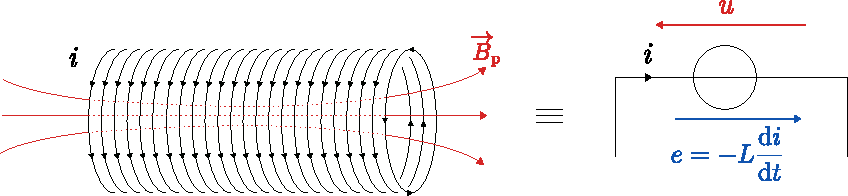
\includegraphics[width=\linewidth]{faraeind}
	\end{center}
\end{tcb*}


\begin{tcb*}(ror){Relation courant-tension d'une bobine}
	\textbf{En l'absence d'autres champs} que le champ propre, on peut donc remplacer
	la bobine par une f.é.m.\ $e_{\rm auto}$ en convention générateur ou $u =
		-e_{\rm auto}$ en convention récepteur, c'est-à-dire
	\psw{%
		\[
			\boxed{u = L \dv{i}{t}}
		\]
	}%
	qui est la caractéristique courant-tension d'une bobine vue en début d'année~!
	\begin{center}
		\sswitch{
			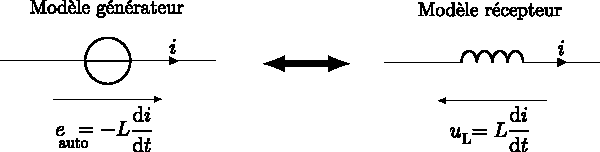
\includegraphics[scale=1, draft=true]{faraequiv}
		}{
			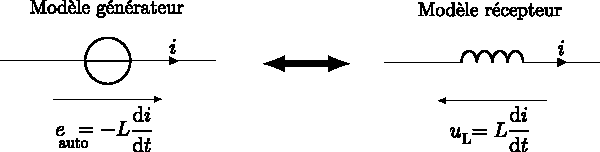
\includegraphics[scale=1]{faraequiv}
		}
		\captionof{figure}{Schémas équivalents générateur/récepteur}
		\label{fig:faraequiv}
	\end{center}
\end{tcb*}


\begin{tcb}(rema)<lftt>'l'{Tension induite par deux sources}
	S'il y a un champ extérieur, on applique la superposition des champs
	magnétiques~:
	\[
		\F\ind{tot} = \F_p + \F\ind{ext}
		\qquad
		\Ra
		\qquad
		e\ind{tot} = -L \dv{i}{t} - \dv{\F\ind{ext}}{t} = e_{\rm auto} + e\ind{ext}
	\]
\end{tcb}

\section{Induction mutuelle}
\label{sec:inducmut}
\subsection{Principe de l'inductance mutuelle}
\label{ssec:prpeinducmut}
\noindent
Soit deux circuits fixes indépendants électriquement, sans champ magnétique
extérieur~:
\smallbreak
\noindent
\begin{minipage}[t]{.6\linewidth}
	\begin{itemize}
		\item Le circuit (1) est parcouru par un courant $i_1$ qui génère un champ
		      magnétique $\vv{B_1}$~;
		\item Le circuit (2) est parcouru par un courant $i_2$ qui génère un champ
		      magnétique $\vv{B_2}$.
	\end{itemize}
	Le champ magnétique total est
	\[
		\vv{B}\ind{tot} =
		\vv{B_1} + \vv{B_2} + \underbracket{\vv{B\ind{ext}}}_{=\vv{0}}
	\]
\end{minipage}
\hfill
\begin{minipage}[t]{.4\linewidth}
	~
	\vspace*{-20pt}
	\begin{center}
		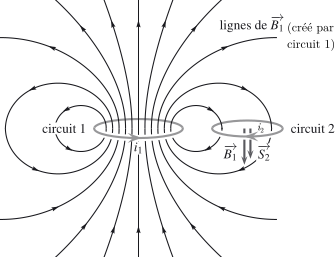
\includegraphics[width=.8\linewidth]{inducmut}
		\label{fig:inducmut}
	\end{center}
\end{minipage}
\textbf{En supposant les champs uniformes}, le flux magnétique total traversant
le circuit (1) est donc~:
\psw{%
	\begin{gather*}
		\F_1 = \vv{B}\ind{tot}\cdot \vv{S_1} =
		\left(\vv{B_1}+\vv{B_2}\right)\cdot \vv{S_1} =
		\vv{B_1}\cdot \vv{S_1}+\vv{B_2}\cdot \vv{S_2}
		\\\Lra
		\F_1 = \F_{p,1} + \F_{2\ra 1}
	\end{gather*}
}%
Avec $\F_p$ le flux propre de chaque circuit, et $\F_{2\ra 1}$ le flux de
$\vv{B_2}$ à travers le circuit (1). De même, en inversant les rôles de (1) et
(2)~:
\psw{%
	\[
		\F_2 = \F_{p,2} + \F_{1\ra 2}
	\]
}%

\begin{tcb*}(prop){Inductance mutuelle}
	\psw{%
		Les flux croisés sont proportionnels au courant les générant, même dans un
		cas non-uniforme, et le coefficient de proportionnalité est \textbf{le même
			pour les deux flux}, et s'appelle \textbf{coefficient d'inductance mutuelle}
		$M$, mesuré en henry~:
		\[
			\boxed{\F_{2\ra 1} = Mi_2}
			\qqet
			\boxed{\F_{1\ra 2} = Mi_1}
		\]
		\vspace*{-10pt}
	}%
\end{tcb*}

\begin{tcb}(rema)<lftt>'l'{Signe de $M$}
	Au contraire de $L$ toujours positive, $M$ peut être positif ou négatif selon
	l'orientation relative des deux circuits.
\end{tcb}

% \paragraph*{Forces électromotrices}
\begin{tcb*}[breakable](appl)<lftt>{Forces électromotrices induites}
	Soit deux circuits non connectés mais en inductance mutuelle. \textbf{Exprimer
		les tensions induites en fonction des intensités et des inductances}.
	\begin{center}
		\sswitch{
			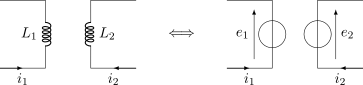
\includegraphics[scale=1, draft=true]{inducmutelec}
		}{
			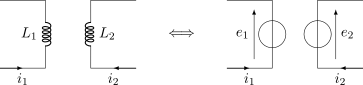
\includegraphics[scale=1]{inducmutelec}
		}
		\captionof{figure}{Circuits en inductance mutuelle.}
		\label{fig:inducmutelec}
	\end{center}
	\tcblower
	Chaque circuit vérifie la loi de \textsc{Faraday}~:
	\psw{%
		\begin{gather*}
			e_1 = - \dv{\F_1}{t} = -\dv{\F_{p,1}}{t} - \dv{\F_{2\ra 1}}{t}
			\qqet
			e_2 = - \dv{\F_2}{t} = -\dv{\F_{p,2}}{t} - \dv{\F_{1\ra 2}}{t}
			\\\Ra
			\left\{%
			\begin{aligned}{}
				\F_{p,1}    & = L_1i_1
				\\
				\F_{2\ra 1} & = Mi_2
			\end{aligned}
			\right.
			\qqet
			\left\{%
			\begin{aligned}{}
				\F_{p,2}    & = L_2i_2
				\\
				\F_{1\ra 2} & = Mi_1
			\end{aligned}
			\right.
			\\\Ra
			\boxed{e_1 = -L_1 \dv{i_1}{t} - M \dv{i_2}{t}}
			\qqet
			\boxed{e_2 = -L_2 \dv{i_2}{t} - M \dv{i_1}{t}}
		\end{gather*}
	}%
\end{tcb*}

\subsection{Bobines imbriquées}
\label{ssec:inducmutimbriq}
On souhaite déterminer l'inductance mutuelle de 2 bobines de même axe, de
longueurs $\ell_{i}$ et de rayons $R_{i}$, parcourues par des intensités $i_{i}$
dirigées dans le même sens. On s'intéresse d'abord à $\F_{2\ra 1}$, le flux créé
par la seconde bobine dans la première.
\begin{figure}[h]
	\centering
	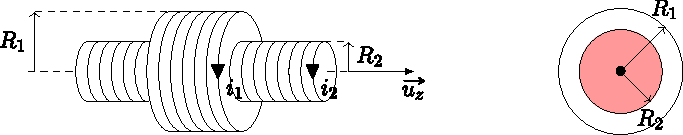
\includegraphics[scale=1]{bobimbriq}
	\label{fig:bobimbriq}
\end{figure}

\paragraph*{Expression du champ magnétique $\vv{B_2}$}~
\smallbreak
\noindent
Le champ magnétique d'une bobine est uniforme en son sein, et négligeable
en dehors, soit
\psw{%
	\[
		\vv{B_2} =
		\left\{%
		\begin{array}{lr}
			\DS
			\mu_0 \frac{N_2}{\ell_2}i_2\,\uz & \quad \text{à l'intérieur}
			\\
			\vv{0}                           & \quad \text{à l'extérieur}
		\end{array}
		\right.
	\]
}%
\vspace{-15pt}

\paragraph*{Flux de $\vv{B_2}$ à travers de $\vv{S_1}$, $\F_{2\to 1}$}~
\smallbreak
\noindent
On oriente $\vv{S_1}$ à partir de $i_1$ par la règle de la main droite~:
\[
	\vv{S_1} = S_1\uz
\]
Or, le champ $\vv{B_2}$ est nul entre $S_2$ et $S_1$, d'où~:
\psw{%
	\begin{align*}
		\F_{2\ra 1} & = \mu_0 \frac{N_2}{\ell_2}i_2 \times S_2\times N_1
		+ 0\times (S_2-S_1) \times N_1
		\\\Lra
		\F_{2\ra 1} & = \mu_0 \frac{N_1N_2S_2}{\ell_2} i_2
		\\\Ra
		\Aboxed{M   & = \mu_0 \frac{N_1N_2S_2}{\ell _2}}
	\end{align*}
}%
\vspace{-15pt}

\paragraph*{Calcul de $\F_{1\ra 2}$}~
\smallbreak
\noindent
Le calcul direct et réel est plus compliqué, puisque les lignes de champs
sortent en réalité de la première bobine et ne sont plus parallèles. On
pourrait se contenter d'utiliser l'inductance mutuelle pour exprimer
directement
\[
	\F_{1\ra 2} = Mi_1
\]
Cependant, avec l'hypothèse de $\vv{B}$ nul en-dehors des bobines, soit
\psw{%
	\[
		\vv{B_1} =
		\left\{%
		\begin{array}{lr}
			\DS
			\mu_0 \frac{N_1}{\ell_1}i_1\,\uz & \quad \text{à l'intérieur}
			\\
			\vv{0}                           & \quad \text{à l'extérieur}
		\end{array}
		\right.
	\]
}%
et toujours avec
\[
	\vv{S_2} = S_2\uz
\]
on voit que la seconde bobine est traversée par $\vv{B_1}$ sur une
\textbf{fraction de sa longueur}, en l'occurrence
\psw{%
	$N_2\times \frac{\ell
			_1}{\ell _2}$. Ainsi,
	\begin{gather*}
		\F_{1\ra 2}  = \mu_0 \frac{N_1}{\cancel{\ell _1}}i_1\times
		S_2 \times N_2\frac{\cancel{\ell _1}}{\ell _2}
		\Lra
		\F_{1\ra 2}  = \mu_0 \frac{N_1N_2S_2}{\ell _2}i_1
	\end{gather*}
}%
Et on retrouve bien $M$.

\begin{tcb*}(rema)<lftt>'l'{Inductance mutuelle en influence totale}
	Si les deux bobines sont de même longueur et même section, alors
	\psw{%
		\begin{gather*}
			M = \mu_0 \frac{N_1N_2}{\ell }S
			\qqav
			L_1 = \mu_0 \frac{N_1{}^{2}}{\ell }S
			\qqet
			L_2 = \mu_0 \frac{N_2{}^{2}}{\ell }S
			\\\Ra
			\boxed{M = \sqrt{L_1L_2}}
		\end{gather*}
	}%
	On parle alors d'«~influence totale~».
\end{tcb*}

\subsection{Circuits électriques couplés par inductance mutuelle}
\label{ssec:inducmutcpl}

\begin{tcb*}(ror){Méthode de résolution}
	\begin{enumerate}
		\item \psw{%
			      Remplacer les inductances par leur f.é.m.\ en \textbf{convention
				      générateur}~;
		      }%
		\item \psw{%
			      Appliquer la loi des mailles pour obtenir les équations électriques~;
		      }%
		\item \psw{%
			      Utiliser la loi de \textsc{Faraday} et exprimer les flux magnétiques en
			      fonction des courants~;
		      }%
		\item \psw{%
			      Résoudre les équations obtenues.
		      }%
	\end{enumerate}
\end{tcb*}

\subsubsection{Étude du circuit}
\label{ssec:mutcpletude}
\noindent
\begin{minipage}[t]{.49\linewidth}
	On étudie le circuit ci-dessous présentant un couplage par induction de deux
	circuits. Le sens de $i_1$ est imposé par le générateur, et le sens de $i_2$
	est conventionnel (selon sa direction, $M$ sera positif ou négatif).
\end{minipage}
\hfill
\begin{minipage}[t]{.49\linewidth}
	~
	\vspace*{-40pt}
	\begin{center}
		\sswitch{
			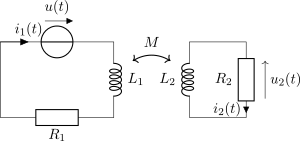
\includegraphics[scale=1, draft=true]{cplmut_a}
		}{
			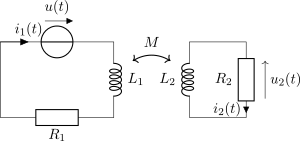
\includegraphics[scale=1]{cplmut_a}
		}
		\captionof{figure}{Circuits couplés.}
		\label{fig:cplmut_a}
	\end{center}
\end{minipage}
\smallbreak

\noindent
\begin{minipage}[c]{.49\linewidth}
	\paragraph*{Circuit équivalent}
	\psw{%
		On remplace les bobines par des générateurs, fléchés en convention générateur
		(à partir du sens de $i_1$ et $i_2$), de forces électromotrices $e =
			-\dd{\F}/\dd{t}$~:
	}
\end{minipage}
\hfill
\begin{minipage}[c]{.49\linewidth}
	\vspace{0pt}
	\begin{center}
		\sswitch{%
			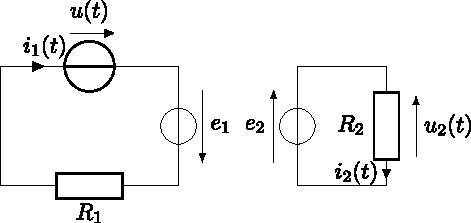
\includegraphics[scale=1, draft=true]{cplmut_b}
			\label{fig:cplmut_b}
		}{%
			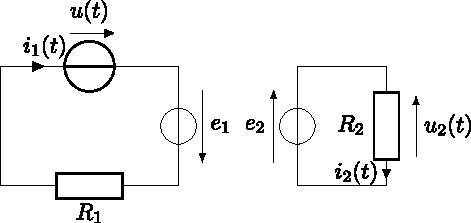
\includegraphics[scale=1]{cplmut_b}
			\label{fig:cplmut_b}
		}%
		\captionof{figure}{Circuit équivalent.}
	\end{center}
\end{minipage}
% \paragraph*{Circuit équivalent}
% \psw{%
% 	On remplace les bobines par des générateurs, fléchés en convention générateur
% 	(à partir du sens de $i_1$ et $i_2$), de forces électromotrices $e =
% 		-\dd{\F}/\dd{t}$~:
% }
% \begin{figure}[h]
% 	\centering
% 	\sswitch{%
% 		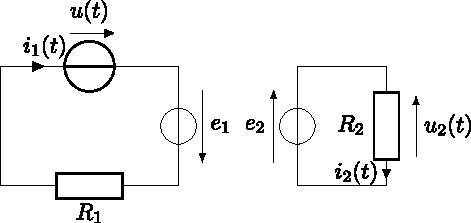
\includegraphics[scale=1, draft=true]{cplmut_b}
% 		\label{fig:cplmut_b}
% 	}{%
% 		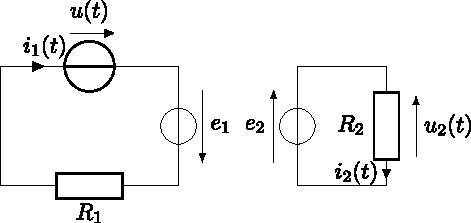
\includegraphics[scale=1]{cplmut_b}
% 		\label{fig:cplmut_b}
% 	}%
% 	\captionof{figure}{Circuit équivalent.}
% \end{figure}
% \vspace*{-10pt}

\vspace{-15pt}
\paragraph*{Équations électriques}~
\smallbreak
\begin{isd}
	\tcbsubtitle{\fatbox{Circuit 1}}
	\psw{%
		\[
			u + e_1 = R_1i_1
		\]
	}%
	\vspace{-15pt}
	\tcblower
	\tcbsubtitle{\fatbox{Circuit 2}}
	\psw{%
		\[
			e_2 = R_2i_2
		\]
	}
	\vspace{-15pt}
\end{isd}

\newpage
\paragraph*{Flux magnétiques et forces électromotrices}~
\smallbreak
\begin{isd}
	\tcbsubtitle{\fatbox{Circuit 1}}
	\psw{%
		\begin{gather*}
			\F_1 = L_1i_1 + Mi_2
			\\\Ra
			e_1 = -\dv{\F_1}{t} = -L_1 \dv{i_1}{t} - M \dv{i_2}{t}
		\end{gather*}
		\vspace*{-10pt}
	}%
	\tcblower
	\tcbsubtitle{\fatbox{Circuit 2}}
	\psw{%
		\begin{gather*}
			\F_2 = L_2i_2 + Mi_1
			\\\Ra
			e_2 = -\dv{\F_2}{t} = -L_2 \dv{i_2}{t} - M \dv{i_1}{t}
		\end{gather*}
		\vspace*{-10pt}
	}%
\end{isd}

\vspace{-15pt}
\paragraph*{Équations couplées}~
\smallbreak
\begin{isd}
	\tcbsubtitle{\fatbox{Circuit 1}}
	\psw{%
		\[
			R_1i_1 + L_1 \dv{i_1}{t} + M \dv{i_2}{t} = u
		\]
	}%
	\vspace{-15pt}
	\tcblower
	\tcbsubtitle{\fatbox{Circuit 2}}
	\psw{%
		\[
			R_2i_2 + L_2 \dv{i_2}{t} + M \dv{i_1}{t} = 0
		\]
	}%
	\vspace{-15pt}
\end{isd}

Ainsi, en l'absence de couplage ($M = 0$), on retrouve les équations d'un
circuit RL classique. Avec le couplage, on peut résoudre ces équations en
passant en RSF~:
\psw{%
	\[
		(R_1 + \jj L_1 \w)\xul{I_1} + \jj M \w \xul{I_2} = \xul{U}
		\qqet
		(R_2 + \jj L_2\w)\xul{I_2} + \jj M\w \xul{I_1} = 0
	\]
}%
On peut alors déterminer le comportement fréquentiel du circuit.

\subsubsection{Bilan énergétique}
\label{ssec:cplnrj}
Pour faire l'étude énergétique du circuit, on procède comme d'habitude en
faisant un bilan de puissance en \textbf{multipliant par $i$} les équations
obtenues par la loi des mailles, ici $i_1$ et $i_2$. À partir des équations
couplées,
\smallbreak
\begin{isd}
	\tcbsubtitle{\fatbox{Circuit 1}}
	\psw{%
	\[
		R_1i_1{}^{2} + L_1i_1 \dv{i_1}{t} + Mi_1 \dv{i_2}{t} = ui_1
	\]
	}%
	\vspace*{-10pt}
	\tcblower
	\tcbsubtitle{\fatbox{Circuit 2}}
	\psw{%
	\[
		R_2i_2{}^{2} + L_2i_2 \dv{i_2}{t} + Mi_2 \dv{i_1}{t} = 0
	\]
	}%
	\vspace*{-10pt}
\end{isd}

Ainsi, par somme on trouve
\psw{%
	\begin{align*}
		R_1i_1{}^{2} +R_2i_2{}^{2} +
		\dv{t}\left( \frac{1}{2} L_1i_1{}^{2} \right) +
		\dv{t}\left( \frac{1}{2}L_2i_2{}^{2} \right) +
		Mi_1 \dv{i_2}{t} + Mi_2 \dv{i_1}{t} =
		ui_1
		\\\Lra
		R_1i_1{}^{2} +R_2i_2{}^{2} +
		\dv{t}\left(
		\frac{1}{2}L_1i_1{}^{2} + \frac{1}{2}L_2i_2{}^{2} + Mi_1i_2
		\right) =
		ui_1
	\end{align*}
}%
\noindent
Ainsi, on met en évidence~:
\begin{itemize}
	\item $\Pc_{J} = R_1i_1{}^{2}(t) + R_2i_2{}^{2}(t)$
	      \psw{%
		      la puissance reçue par les résistances (dissipée par effet Joule)~;
	      }%
	\item $\Pc\ind{mag} = \dv{t}
		      \left(
		      \frac{1}{2}L_1i_1{}^{2} + \frac{1}{2}L_2i_2{}^{2} + Mi_1(t)i_2(t)
		      \right)$
	      \psw{%
		      la puissance magnétique stockée dans les deux circuits~;
	      }%
	\item $\Pc_{g} = u(t)i_1(t)$
	      \psw{%
		      la puissance fournie par le générateur.
	      }%
\end{itemize}
\begin{tcb*}[breakable](ror){Bilan énergétique}
	\begin{center}
		L'énergie du champ magnétique créé par deux circuits couplés par induction
		mutuelle est
	\end{center}
	\psw{%
	\[
		\boxed{\Ec\ind{mag} =
		\frac{1}{2}L_1i_1{}^{2} +
		\frac{1}{2}L_2i_2{}^{2} +
		Mi_1i_2
		}%
	\]
	}%
	\begin{itemize}
		\item
		      \psw{%
		      $L_1i_1{}^{2}/2$ est l'énergie magnétique emmagasinée dans le premier
		      circuit~;
		      }%
		\item
		      \psw{%
		      $L_2i_2{}^{2}/2$ est l'énergie magnétique emmagasinée dans le second
		      circuit~;
		      }%
		\item
		      \psw{%
			      $Mi_1i_2$ représente l'\textbf{énergie de couplage magnétique} entre
			      les deux circuits.
		      }%
	\end{itemize}
\end{tcb*}

\section{Applications}
\label{ssec:cplimpl}
\subsection{Quelques exemples}

\begin{itemize}
	\item[b]{Radio-identification}: placée dans des étiquettes adhésives comme
	dans les antivols par exemple, un courant sera induit dans le circuit s'il
	passe à côté d'un système actif fournissant un champ magnétique. Ce courant
	alimente alors une petite antenne envoyant l'information de la puce (dite
	RFID pour \textit{radio frequency identification}).
	\item[b]{Détecteur de métaux, boucles magnétiques (péages, parking)}: une
	bobine créé un champ magnétique et, si un morceau de métal se trouve à
	proximité, il se créé un courant en son sein. Ce courant créé lui-même un
	champ magnétique qui perturbe le circuit primaire.
	\item[b]{Rechargement par induction (brosses à dent, portables)}: le chargeur
	est muni d'une bobine qui créé un champ qui va induire un champ dans un second
	circuit.
	\item[b]{Chauffage par induction}: le courant généré dans le second circuit se
	réparti dans tout le volume~; on les appelle \textbf{courants de
		\textsc{Foucault}}. Ils permettent le chauffage par effet \textsc{Joule}.
\end{itemize}

\subsection{Transformateur}
En enroulant deux bobines différentes
autour d'un noyau de métal canalisant le flux, on peut \textbf{diminuer ou
	augmenter la tension} d'un circuit à l'autre.

\subsubsection{Constitution}

\begin{tcb*}(defi){Transformateur}
	Un transformateur monophasé est constitué d'un matériau ferromagnétique sur
	lequel sont bobinés deux enroulements électriques, indépendants
	électriquement (masses séparées)~:
	\begin{itemize}
		\item[b]{Enroulement primaire}: relié à la source d'alimentation (on notera
		les grandeurs $u_1$, $i_1$ etc.)
		\item[b]{Enroulement secondaire}: relié à la charge (noté $u_2$, $i_2$
		etc.)
	\end{itemize}
	\noindent
	\begin{minipage}[c]{.49\linewidth}
		\begin{center}
			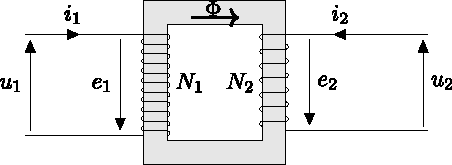
\includegraphics[scale=1]{transfo_a.pdf}
			\captionof{figure}{Représentation complète}
		\end{center}
	\end{minipage}
	\hfill
	\begin{minipage}[c]{.49\linewidth}
		\begin{center}
			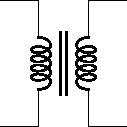
\includegraphics[scale=1]{transfo_c.pdf}
			\captionof{figure}{Schématisation électrique}
		\end{center}
	\end{minipage}
\end{tcb*}

Le rôle du circuit magnétique est d'assurer une canalisation optimale des lignes
de champ magnétique afin d'obtenir un couplage maximal entre les deux
enroulements. Cela veut dire que le flux magnétique traversant une spire du
circuit 1 est égal à celui traversant une spire du circuit 2.

\begin{tcb*}(defi){Transformateur parfait}
	Dans le modèle du transformateur parfait~:
	\begin{itemize}
		\item \psw{la résistance des enroulements est négligée~;}
		\item \psw{il n'y a pas de perte de flux magnétique entre les enroulements}
	\end{itemize}
\end{tcb*}

\vspace{-10pt}
\subsubsection{Loi des tensions}

\begin{tcb*}(prop){Loi des tensions}
	Dans un transformateur parfait, les tensions au primaire et au secondaire sont
	telles que~:
	\psw{%
		\[
			\boxed{\frac{u_2 (t)}{u_1 (t)} = \frac{N_2}{N_1} = m}
		\]
	}%
	où $m$ est le \textbf{rapport de transformation}.
\end{tcb*}

\begin{tcb*}(demo){Loi des tensions}
	Le flux à travers une spire au primaire est égal à celui dans une spire du
	secondaire. Ainsi, le flux total à travers les enroulements sont~:
	\psw{%
		\[
			\F_{1, \mathrm{tot}} = N_1 \F
			\qqet
			\F_{2, \mathrm{tot}} = N_2 \F
			\qqav
			\F = BS
		\]
	}%
	Ainsi, les forces électromotrices sont~:
	\smallbreak
	\begin{isd}
		\tcbsubtitle{\fatbox{Circuit 1}}
		\psw{%
			\begin{align*}
				e_1 = -\dv{\F_{1,\mathrm{tot}}}{t} & = -N_1 \dv{\F}{t}
				\\\Lra
				u_1                                & = N_1 \dv{\F}{t}
			\end{align*}
		}%
		\vspace{-15pt}
		\tcblower
		\tcbsubtitle{\fatbox{Circuit 2}}
		\psw{%
			\begin{align*}
				e_2 = -\dv{\F_{2,\mathrm{tot}}}{t} & = -N_2 \dv{\F}{t}
				\\\Lra
				u_2                                & = N_2 \dv{\F}{t}
			\end{align*}
		}%
		\vspace{-15pt}
	\end{isd}
	D'où le résultat en divisant.
\end{tcb*}

\begin{tcb}(rema)<lftt>{Différents transformateurs}
	\begin{itemize}
		\item Lorsque la tension au secondaire est plus élevée qu'au primaire, on
		      parle d'\textbf{élévateur de tension} (à la sortie d'une centrale par
		      exemple).
		\item Dans le cas contraire, on parle d'\textbf{abaisseur de tension}
		      (transformateur de quartier par exemple).
		\item Il existe aussi des transformateurs où la tension est identique au
		      primaire et au secondaire~: un tel transformateur est appelé
		      \textbf{transformateur d'isolement} et permet d'isoler la masse de la terre~;
		      on évite ainsi des électrocutions en milieu humide (salle de bain par
		      exemple).
	\end{itemize}
\end{tcb}

\begin{tcb*}(impo){Transformateur}
	\begin{center}
		Tout ceci n'est valable que pour un champ variable, par pour des tensions
		constantes~!
	\end{center}
\end{tcb*}

\subsubsection{Loi des courants}
\label{sssec:label}

\begin{tcb*}(prop){Loi des courants}
	Dans un transformateur parfait, les courants au primaire et au secondaire sont
	tels que~:
	\psw{%
		\[
			\boxed{\frac{i_2 (t)}{i_1 (t)} = - \frac{N_1}{N_2} = -\frac{1}{m}}
		\]
	}%
\end{tcb*}

\begin{tcb*}(demo){Loi des courants}
	Si le transformateur est idéal, il transfert la totalité de la puissance électrique. Or, on a
	\psw{%
		\begin{gather*}
			\Pc_r = u_1i_1
			\qqet
			\Pc_f = -u_2i_1
			\\\beforetext{$\Pc_r = \Pc_f \Ra$}
			u_1 i_1 = -u_2 i_2
			\Lra
			\boxed{\frac{i_2}{i_1} = - \frac{u_1}{u_2}}
			\qed
		\end{gather*}
	}%
\end{tcb*}

\begin{tcb}(rema)<lftt>{Signe du rapport}
	Le signe a peu d'importance car un transformateur fonctionne avec des tensions
	alternatives. Il dépend du sens de l'enroulement choisi sur le schéma
	(arbitrairement). Seule la valeur efficace nous intéresse.
\end{tcb}

\end{document}
